\section{Конструкторский раздел}
Во время разработки программы, должна быть учтена возможность её модификации. Объектно-ориентированный подход обеспечивает гибкость в вопросе изменения уже существующего кода \cite{bib:oop_mod}.

В программы будет высоконагруженная секция --- алгоритм отрисовки сцены. При разработке алгоритма, необходимо как можно больше операций перенести на другие части программы, с целью получения максимального выигрыша в производительности.

\subsection{Сцена, объекты сцены}
Определим ключевые сущности, тем или иным образом связанные с понятием сцены:
\begin{itemize}
	\item Сцена. Должна агрегировать все объекты, которые могут быть включены в неё.
	\item Полигональная модель. Будет содержать множество точек в пространстве и ими задаваемые треугольники.
	\item Камера. Представляет собой точку в пространстве, имеющую направление и область обзора.
	\item Кубик Рубика. Агрегирует 27 моделей малых параллелограммов, формирующих зеркальный кубик Рубика.
\end{itemize}

Добавив несколько вспомогательных классов, получим UML-диаграмму (см. рис. \ref{fig:uml_scene}). Полученая диаграмма описывает некий домен сцены. Рассмотрим основные математические структуры:
\begin{figure}[ht]
	\centering
	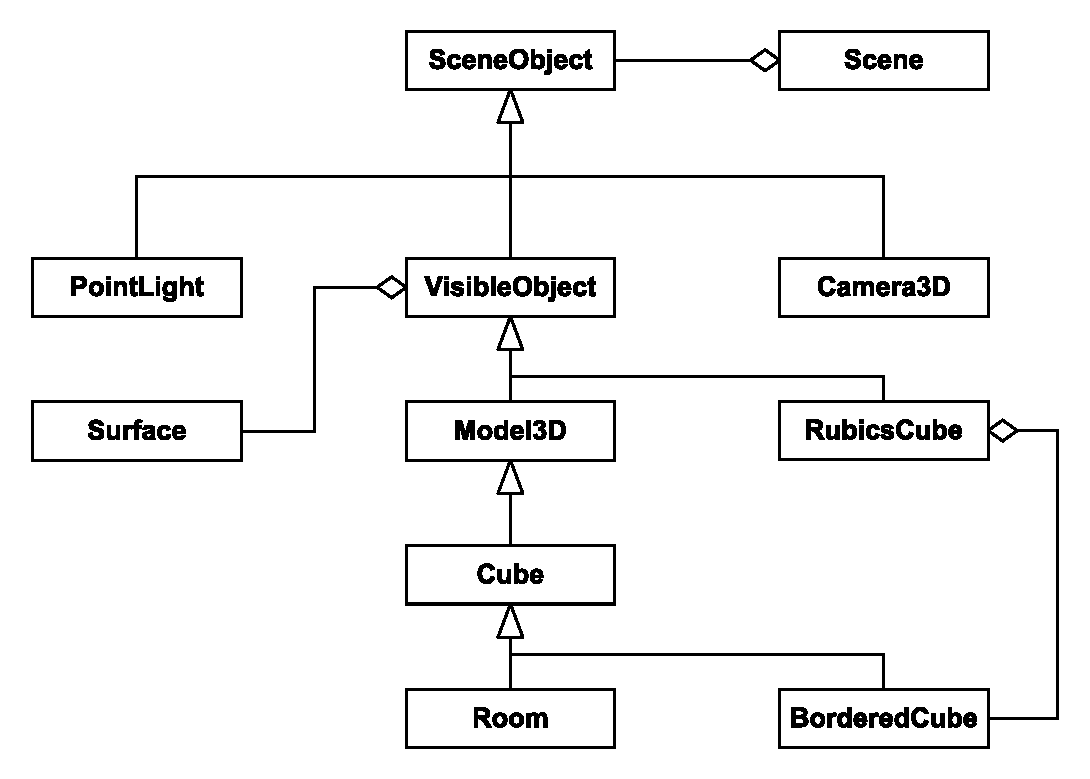
\includegraphics[width=1\linewidth]{uml_scene}
	\caption{UML диаграмма классов сцены, без описания полей и методов}
	\label{fig:uml_scene}
\end{figure}

\subsection{Математические структуры}
Для описания положения объекта в пространстве, необходима следующая информация:
\begin{itemize}
	\item позиция объекта,
	\item поворот объекта,
	\item размер объекта.
\end{itemize}

\subsubsection{Трёхмерный вектор}
Трёхмерный вектор является тройкой действительных чисел $(x, y, z)$, каждая компонента которого является величиной проекции на соответствующую ось \cite{bib:vector}.

Позиция объекта может быть описана радиус-вектором, описывающим смещение всех точек объекта относительно начала координат. Таким образом, достаточно прибавить данный радиус-вектор к каждой точке трёхмерной модели, чтобы получить её истинное положение.

Используя точно такую же структуру, будем обозначить размер объекта. Каждый компонент вектора является коэффициентом масштабирования для каждой оси.

\subsubsection{Кватернион}
Использование тройки углов, описывающих последовательный поворот объекта вдоль всех осей, имеет свои недостатки \cite{bib:euler_problems}:
\begin{itemize}
	\item неоднозначность. Для любой последовательности вращений $A$, существует как минимум одна другая последовательность, приводящая объект к тому-же положению, что $A$;
	\item некорректный результат при последовательном применении двух и более троек углов поворота.
\end{itemize}

Вместо так называемых Эйлеровых углов, предпочтительнее использовать кватернионы \cite{bib:quaternions}.

Кватернион представляет собой кортеж из четырёх чисел $(q_0, q_1, q_2, q_3)$. Для каждого кватерниона $q$, существует обратный ему $q^{-1}\ne q$:
\begin{equation}
	q^{-1}=(q_0, -q_1, -q_2, -q_3),
\end{equation}

исключением является единичный кватернион $(1, 0, 0, 0)$, так как он обратен самому себе.

Для кватернионов определена операция умножения. Пусть:
\begin{equation}
	(t_0, t_1, t_2, t_3) = (r_0, r_1, r_2, r_3)\times(s_0, s_1, s_2, s_3).
\end{equation}

Тогда:
\begin{subequations}
	\begin{align}
		t_0=(r_0\cdot s_0-r_1\cdot s_1-r_2\cdot s_2-r_3\cdot s_3) \\
		t_1=(r_0\cdot s_1+r_1\cdot s_0-r_2\cdot s_3+r_3\cdot s_2) \\
		t_2=(r_0\cdot s_2+r_1\cdot s_3+r_2\cdot s_0-r_3\cdot s_1) \\
		t_3=(r_0\cdot s_3-r_1\cdot s_2+r_2\cdot s_1+r_3\cdot s_0)
	\end{align}
\end{subequations}

С помощью кватерниона, можно повернуть точку в пространстве, заданную тремя координатами. Для этого нужно задать кватернион $p$, как:
\begin{equation}
	p=(p_0,p_1,p_2,p_3)=(0, x, y, z),
\end{equation}
где $(x, y, z)$ - точка в пространстве. Получим $p'$ следующим образом:
\begin{equation}
	p'=q^{-1}\cdot p\cdot q,
\end{equation}
где $q$ --- кватернион, описывающий вращение. Искомая точка является тройкой $(p'_1, p'_2, p'_3)$.

\subsubsection{Цвет}
Структура цвета необходима для описания поверхностей объектов. Представляет собой тройку чисел $(r, g, b)$. Значение компонент определяет интенсивность цветов: красного, зелёного и синего соответственно. Сочетания этих трёх цветов разной интенсивности позволяют получить любой другой цвет.

Определим операцию умножения цвета на скаляр:
\begin{equation}
	C\cdot k=(r, g, b)\cdot k=(r\cdot k, g\cdot k, b\cdot k),
\end{equation}
где $C$ --- исходный цвет, $k$ --- скаляр.

Определим операцию сложения цветов:
\begin{equation}
	C_1+C_2=(r_1, g_1, b_1)+(r_2, g_2, b_2)=(r_1+r_2,g_1+g_2,b_1+b_2),
\end{equation}
где $C_1$ и $C_1$ --- исходные цвета

\subsubsection{Список математических структур}
В конечном итоге, выделяем следующие структуры:
\begin{itemize}
	\item Vector3D --- трёхмерный вектор
	\item Quaternion --- кватернион
	\item Transform --- положение объекта в пространстве
	\item Color --- цвет
\end{itemize}

\subsection{Алгоритм обратной трассировки лучей}
Основная идея алгоритма трассировки лучей заключается в том, чтобы проследить путь, который проходит свет от источника до наблюдателя. Делается этот процесс в обратном направлении, то есть из точки наблюдателя выпускаются лучи, которые, несколько раз отражаются от встреченных поверхностей. Данный процесс продолжается до тех пор, пока либо количество дополнительно выпущеных лучей не превысит определённое значение, либо очередная поверхность не окажется неотражающей.

\subsubsection{Алгоритм определения цвета пикселя}
Алгоритм, определяющий цвет пикселя, принимает на вход два трёхмерных вектора: местонахождение наблюдателя (rs) и направление бросания луча (rd). Схема алгоритма представлена на рис. \ref{fig:calculate_pixel_color}

\begin{figure}[!ht]
	\centering
	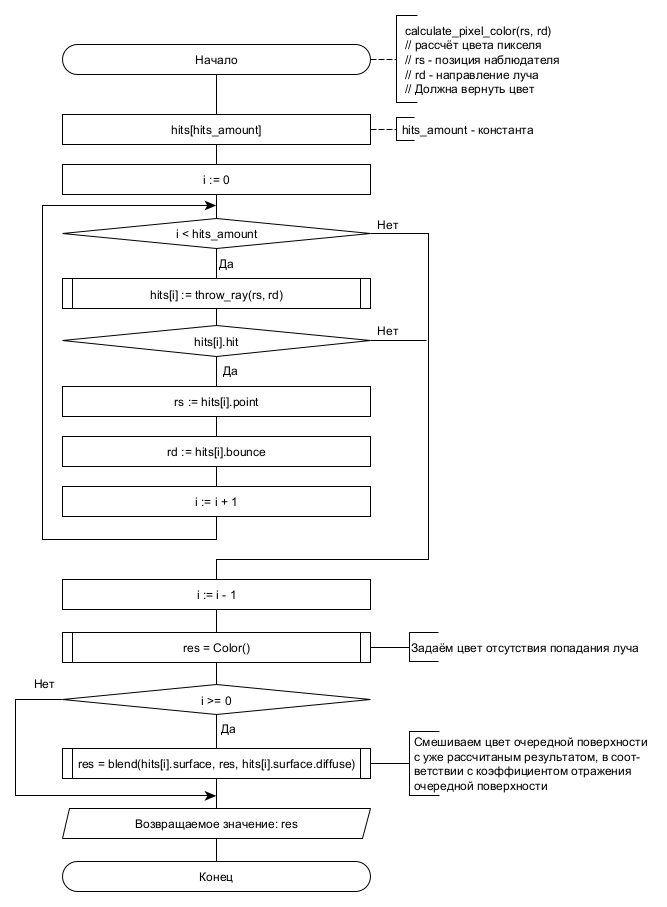
\includegraphics[width=1\linewidth]{calculate_pixel_color}
	\caption{Схема алгоритма определения цвета пикселя}
	\label{fig:calculate_pixel_color}
\end{figure}

Переменная hits[] является массивом из структур, содержащих информацию о попадании. Они должны хранить следующие данные:
\begin{itemize}
	\item было ли попадание (hit) --- логическое;
	\item точке попадания луча (point) --- трёхмерный вектор;
	\item направление отскока (bounce) --- трёхмерный вектор;
	\item поверхность, с которой произошло пересечение (surface) --- поверхность;
\end{itemize}

Структура поверхности содержит в себе информацию о треугольнике в пространстве и его свойствах, а именно:
\begin{itemize}
	\item три точки, задающие треугольник (points) --- тройка трёхмерных векторов;
	\item коэффициент рассеивания (diffuse) --- вещественное. Является обратным к коэффициенту отражения;
	\item цвет поверхности (color) – цвет;
	\item нормаль к поверхности (normal) --- трёхмерный вектор;
	\item объект, частью которого является поверхность (owner) --- объект сцены;
\end{itemize}

Функция Blend реализует смешение двух цветов по формуле:
\begin{equation}
	C = C_1\cdot k+C_2\cdot(1-k),
\end{equation}
где $C$, $C_1$, $C_2$ --- цвета, $k\in[0, 1]$ --- скаляр.

\subsubsection{Алгоритм бросания луча}
Алгоритм бросания луча принимает на вход два трёхмерных вектора: местонахождение наблюдателя (rs) и направление бросания луча (rd). Схема алгоритма представлена на рис. \ref{fig:throw_ray}.

\begin{figure}[!ht]
	\center{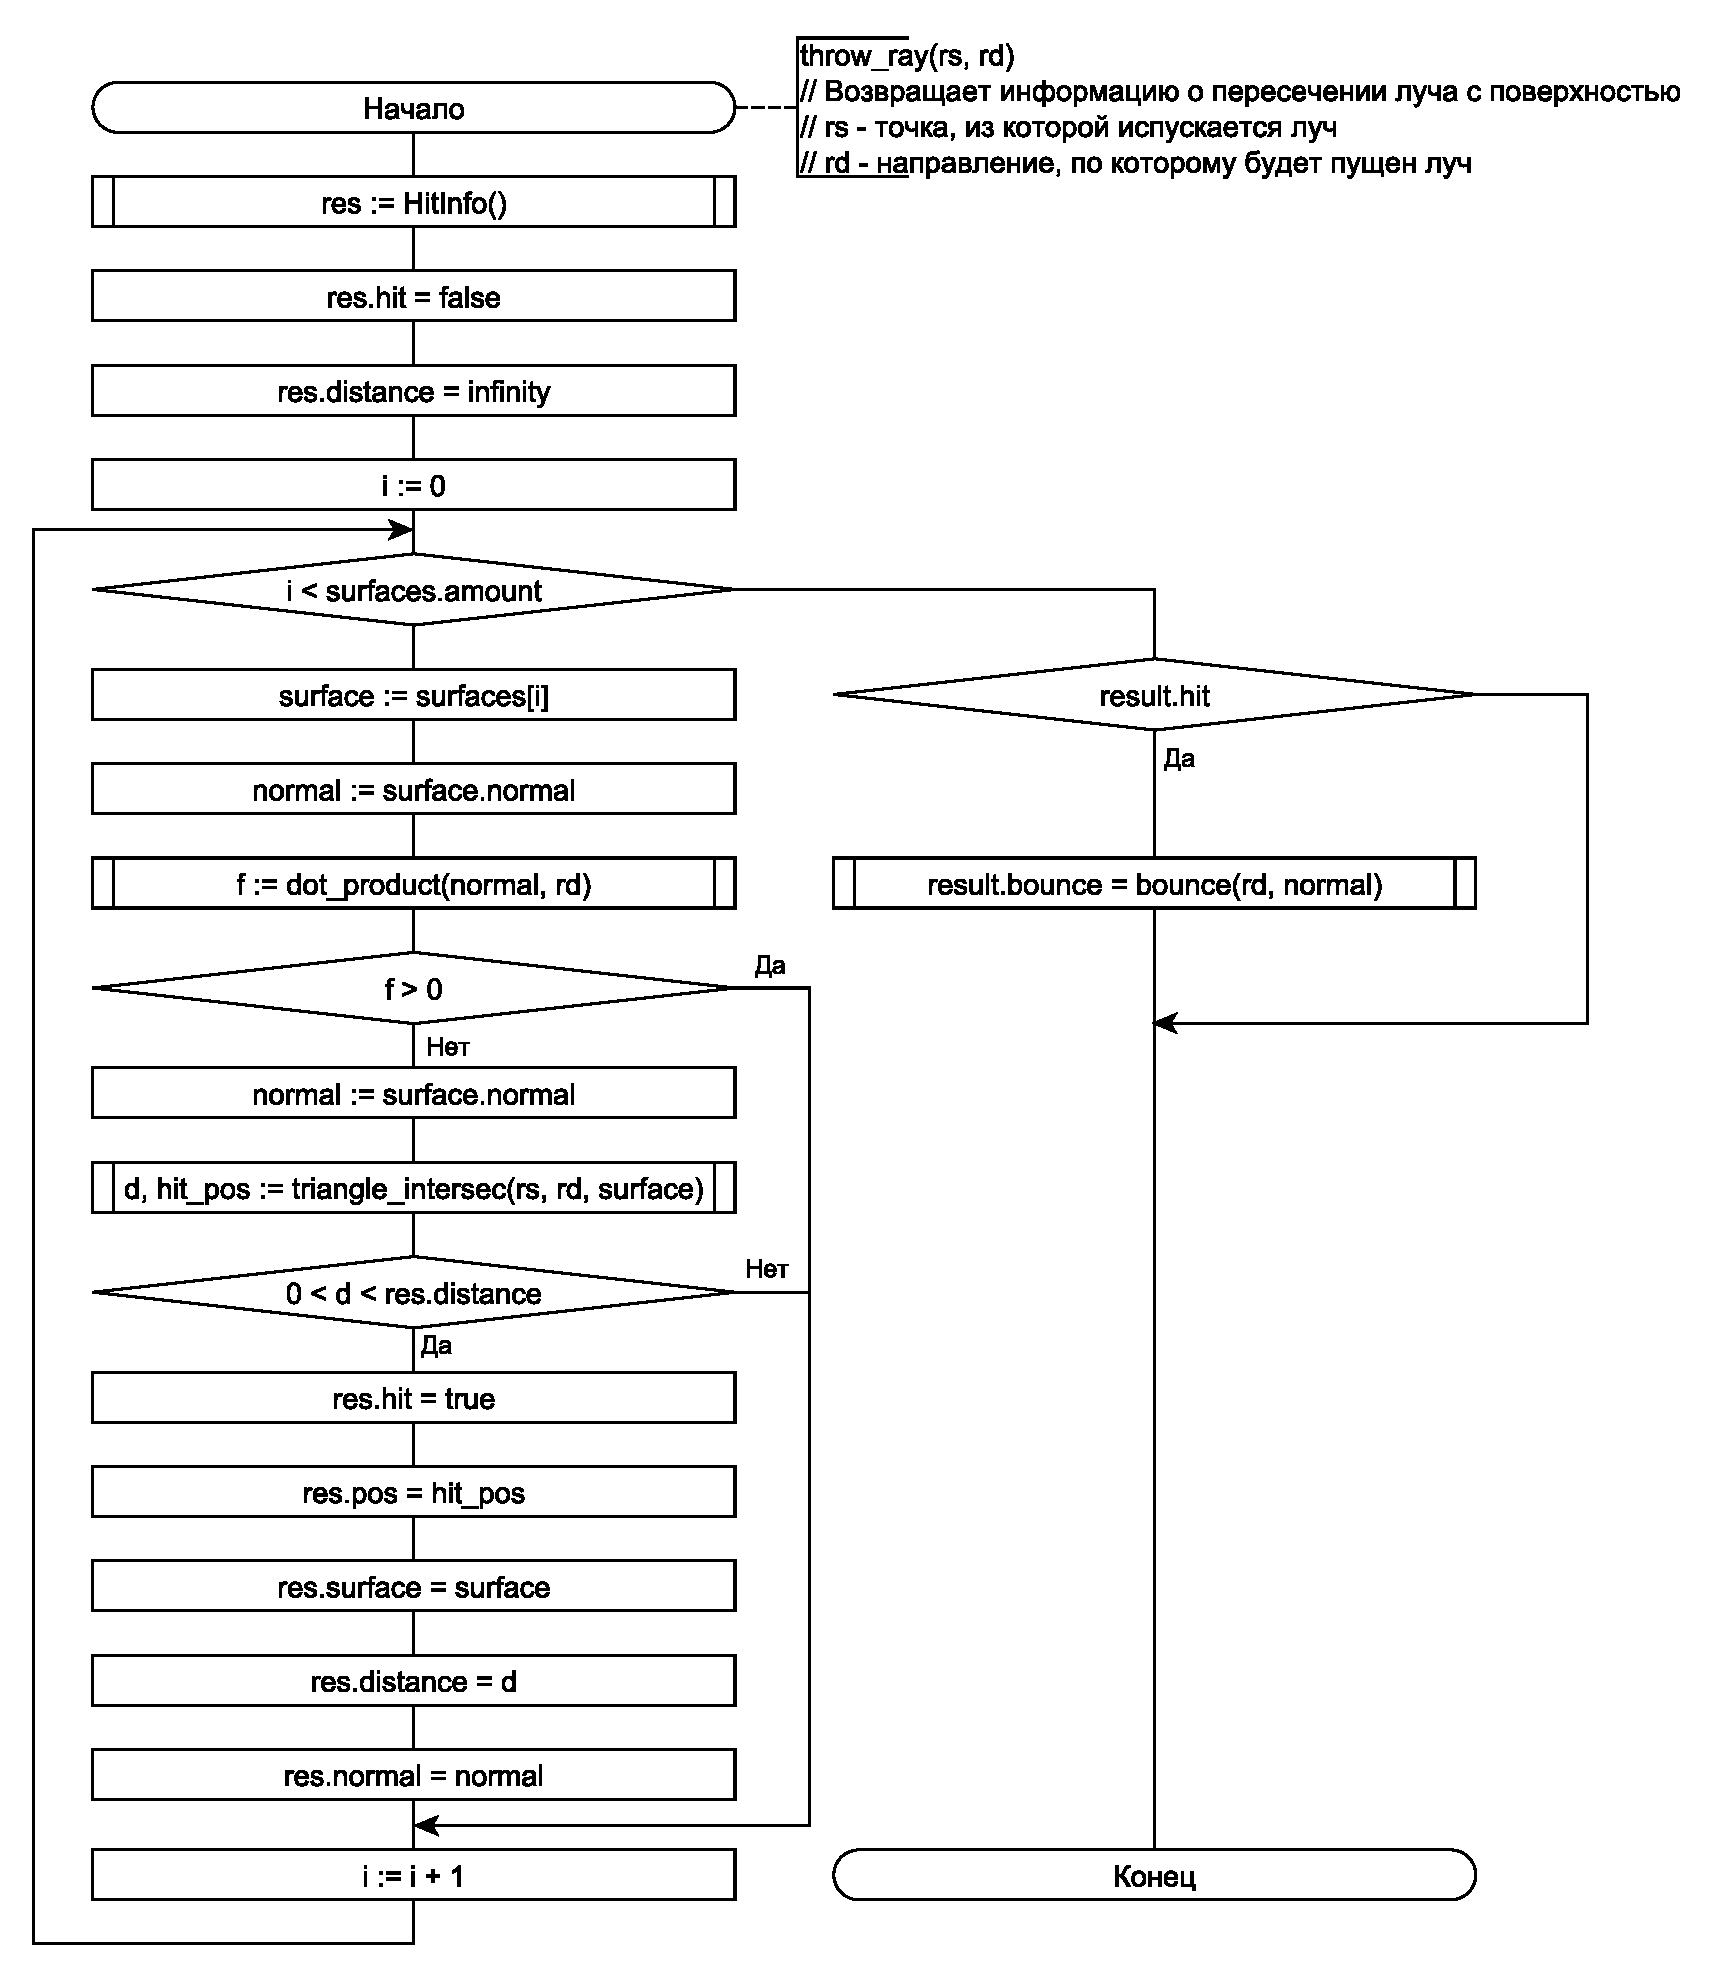
\includegraphics[width=1\linewidth]{throw_ray}}
	\caption{Схема алгоритма бросания луча}
	\label{fig:throw_ray}
\end{figure}

Функция bounce выполняет отражение вектора $\bar V$ относительно нормали $\bar n$ в соответствии с формулой \ref{eq:bounce}

\subsubsection{Алгоритм поиска пересечения луча с треугольником}
В качестве алгоритма поиска пересечения луча с треугольником используется алгоритм Моллера-Трумбора\cite{bib:mollertrumbor}. Схема алгоритма представлена на рис. \ref{fig:triangle_intersec}
\begin{figure}[!ht]
	\center{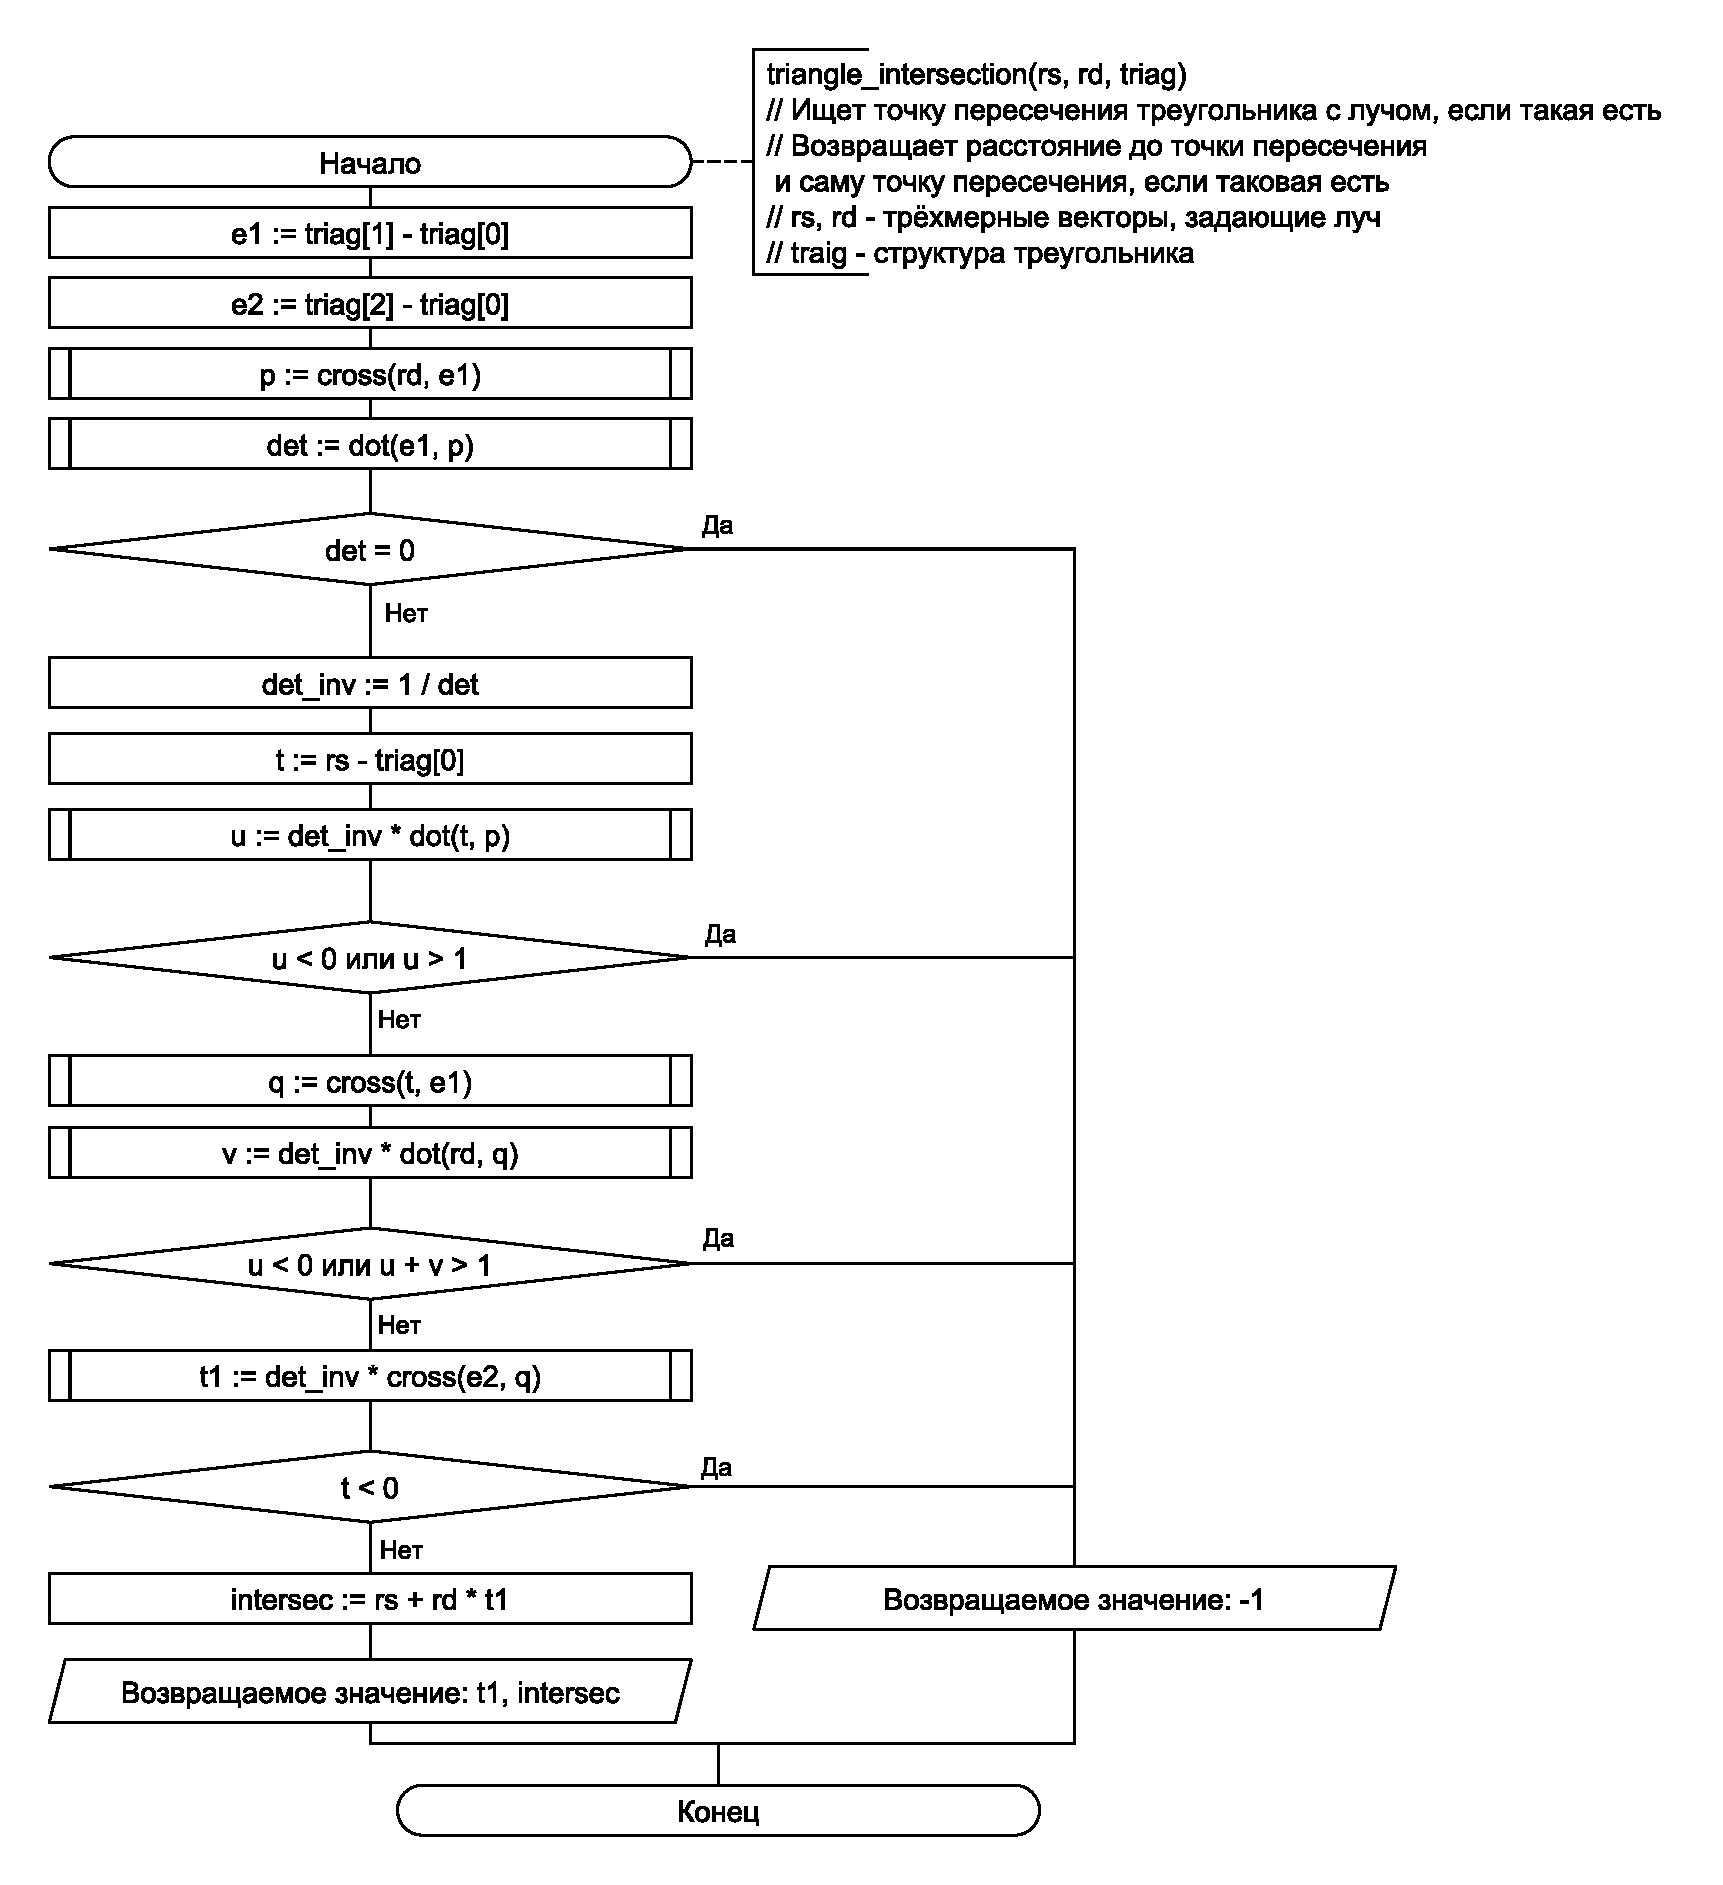
\includegraphics[width=1\linewidth]{triangle_intersec}}
	\caption{Схема алгоритма поиска пересечения луча с треугольником}
	\label{fig:triangle_intersec}
\end{figure}

Функция cross выполняет векторное произведение двух векторов по формуле:
\begin{equation}
	(x_1, y_1, z_1)\times(x_2, y_2, z_2)=(y_1\cdot z_2-z_1\cdot y_2,~z_1\cdot x_2-x_1\cdot z_2,~x_1\cdot y_2-y_1\cdot x_2)
\end{equation}

Функция dot вычисляет скалярное произведение двух векторов по формуле:
\begin{equation}
	(x_1, y_1, z_1)\cdot(x_2, y_2, z_2) = x_1\cdot x_2+y_1\cdot y_2+z_1\cdot z_2
\end{equation}

Идея алгоритма заключается в том, чтобы отыскать точку пересечения луча с треугольником в барицентрических координатах. Вместо того, чтобы искать точку пересечения луча и плоскости, а потом определять лежит ли точка внутри треугольника, получив барицентрические координаты по их значению можно сразу понять, лежит ли точка внутри треугольника или нет

\subsection{Зеркальный кубик Рубика}
\subsubsection{Создание зеркального кубика Рубика}
Создавать зеркальный кубик Рубика необходимо в соответствии с пропорциями, указанными на рис. \ref{fig:mirrored_cube_proportions}. Схема алгоритма создания параллелограммов представлена на рис \ref{fig:rubicks_create}.

\begin{figure}[!ht]
	\center{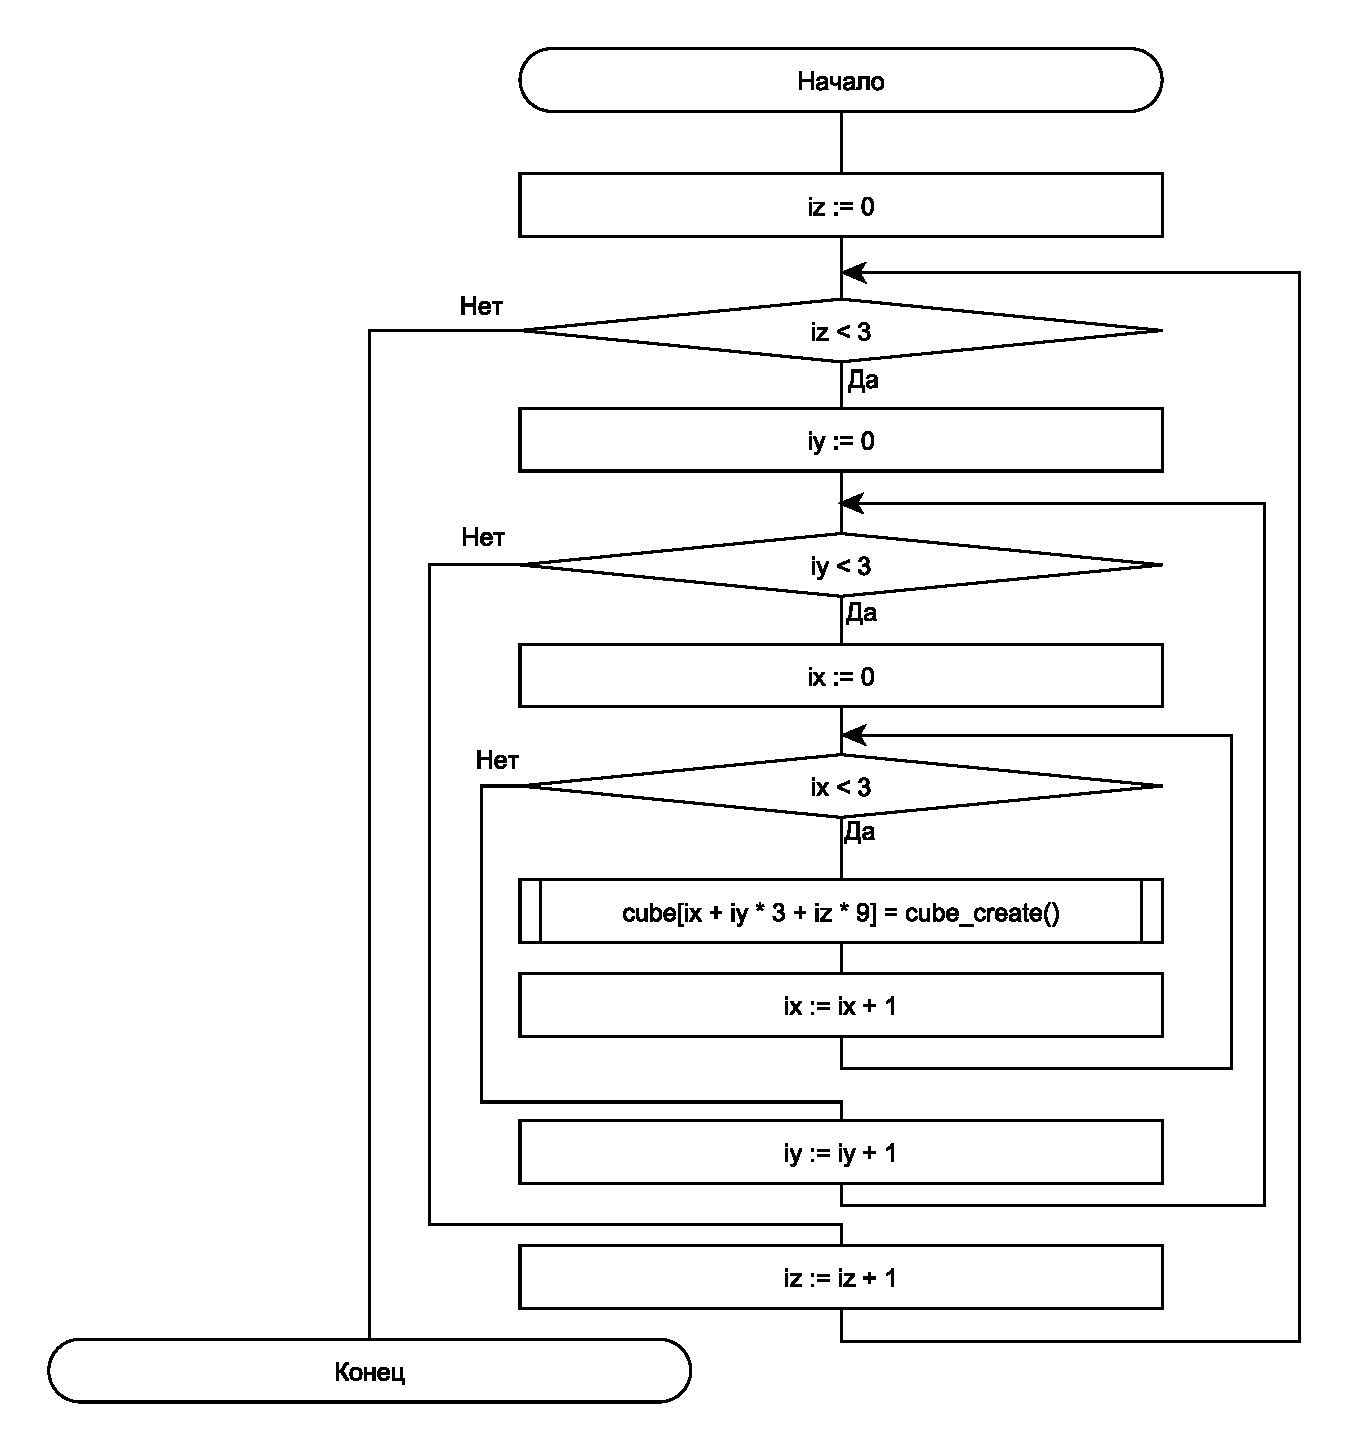
\includegraphics[width=1\linewidth]{rubicks_create}}
	\caption{Схема алгоритма создания кубика рубика}
	\label{fig:rubicks_create}
\end{figure}

Данная схема не иллюстрирует использование пропорций, и отражает лишь порядок в котором должны создаваться параллелограммы.

\subsubsection{Вращение зеркального кубика Рубика}

Вращение грани производится в три этапа (порядок произвольный):
\begin{enumerate}
	\item вращение моделей,
	\item смещение граней в массиве,
	\item смещение углов в массиве.
\end{enumerate}

Под углами и гранями подразумеваются угловые и граневые параллелограммы кубика Рубика.

Смещение граней и углов в массиве выполняется как циклический сдвиг его элементов с соответствующей четвёркой индексов. В таблице \ref{tabular:cube_indexes} поставлены в соответствие какой циклический сдвиг нужно сделать при повороте соответствующей грани. Если вращение выполняется в противоположную сторону, достаточно развернуть последовательность индексов в другую сторону.

\begin{table}
	\centering
	\caption{грани кубика Рубика и соответствующие им параллелограммы}
	\label{tabular:cube_indexes}
	\begin{tabular}{|c|c|c|}
		\hline
		Сторона & Индексы углов & Индексы граней \\
		\hline
		\hline
		F & 0, 6, 24, 18	& 3, 15, 21, 9		\\ \hline
		B & 8, 2, 20, 26	& 5, 11, 23, 17		\\ \hline
		L & 6, 8, 26, 24	& 7, 17, 25, 15		\\ \hline
		R & 2, 0, 18, 20	& 1, 9, 19, 11		\\ \hline
		U & 18, 24, 26, 20	& 21, 25, 23, 19	\\ \hline
		D & 0, 2, 8, 6		& 1, 5, 7, 3		\\ \hline
	\end{tabular}
\end{table}

\subsection{Вывод по разделу}
В конструкторском разделе была описана архитектура создаваемой программы;
выделены структуры, используемые в программе;
ключевые алгоритмы, в числе которых отрисовка сцены методом трассировки лучей,
поиск точки пересечения луча и треугольника, вращение кубика Рубика.

